\documentclass[tikz,border=5pt]{standalone}
\usetikzlibrary{bending,patterns}
\usepackage{fourier}
\begin{document}
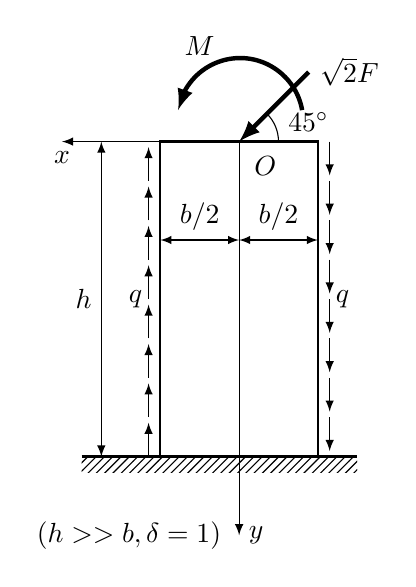
\begin{tikzpicture}[>=latex]
    \draw[->] (1,0) -- (-2.25,0) node[below] {$x$};
    \draw[->] (0,0) node[below right=2pt] {$O$} -- (0,-5) node[right] {$y$} node[left=3pt] {($h>>b,\delta=1$)};
    \draw[thick] (1,0) rectangle (-1,-4);
    \draw[ultra thick,-latex] (45:1.25) node[right] {$\sqrt{2}F$} -- (0,0);
    \draw (.5,0) node[above right] {$45^\circ$} arc (0:45:.5);
    \draw[ultra thick,->] (.8,.4) arc (10:170:.8) node[pos=.75,above=2pt] {$M$};
    \draw[<->] (-1.75,0) -- node[left] {$h$} ++(0,-4);
    \fill[pattern=north east lines] (-2,-4.2) rectangle (1.5,-4);
    \draw[thick] (-2,-4) -- (1.5,-4);
    \draw[<->] (1,-1.25) -- node[above] {$b/2$} (0,-1.25);
    \draw[<->] (-1,-1.25) -- node[above] {$b/2$} (0,-1.25);
    \path 
        (-1,0) -- node[left=3pt] {$q$} ++(0,-4)
        (+1,0) -- node[right=3pt] {$q$} ++(0,-4)
    ;
    \foreach \yy in {0,-.5,...,-3.5} {
        \draw[->,shorten >=2pt] (1.15,\yy) -- ++(0,-.5);
        \draw[->,shorten >=2pt] (-1.15,{-4-\yy}) -- ++(0,.5);
    }
\end{tikzpicture}

\end{document}